\documentclass[twocolumn,11pt]{article}
\usepackage[utf8]{inputenc}
\usepackage[T1]{fontenc}
\usepackage[english]{babel}
\usepackage[a4paper,margin=2.0cm]{geometry}
\usepackage{amsmath,amssymb,amsfonts}
\usepackage{graphicx}
\usepackage{booktabs}
\usepackage{multirow}
\usepackage{array}
\usepackage{url}
\usepackage{hyperref}
\usepackage[numbers,sort&compress]{natbib}
\usepackage{xcolor}
\usepackage{tikz}
\usepackage{pgfplots}
\pgfplotsset{compat=1.18}
\usetikzlibrary{patterns,positioning,shapes.geometric,arrows.meta,calc}
\usepackage{caption}
\usepackage{subcaption}
\usepackage{authblk}
\usepackage{titlesec}
\usepackage{enumitem}
\titleformat{\section}{\normalfont\large\bfseries}{\thesection}{1em}{}
\titleformat{\subsection}{\normalfont\normalsize\bfseries}{\thesubsection}{1em}{}
\definecolor{vibrantblue}{RGB}{0,119,187}
\definecolor{vibrantcyan}{RGB}{51,187,238}
\definecolor{vibrantteal}{RGB}{0,153,136}
\definecolor{vibrantorange}{RGB}{238,119,51}
\definecolor{vibrantred}{RGB}{204,51,17}
\definecolor{vibrantmagenta}{RGB}{238,51,119}
\definecolor{vibrantgrey}{RGB}{187,187,187}
\hypersetup{colorlinks=true,linkcolor=vibrantblue,citecolor=vibrantteal,urlcolor=vibrantblue}
\title{\vspace{-1.2cm}\Large\textbf{SimilCode: A Web-Based System for Multidimensional Source Code Similarity Detection and Algorithmic Efficiency Analysis Using Generative Artificial Intelligence}}
\author[1]{Gleiston C. Guerrero-Ulloa}
\author[1]{Rafael A. Navas-Rivera}
\author[1]{Efra\'in-D\'iaz Mac\'ias}
\author[2]{Carlos Rodr\'iguez Dominguez}
\author[2]{Miguel J. Hornos\thanks{Corresponding author. E-mail: mhornos@ugr.es}
}
\affil[1]{Faculty of Computer Sciences, Universidad T\'ecnica Estatal de Quevedo, Quevedo 120501, Ecuador}
\affil[2]{Software Engineering Department, University of Granada, Granada 18014, Spain}
\date{}
\begin{document}
    \twocolumn[
    \begin{@twocolumnfalse}
    \maketitle
    \begin{abstract}
    \noindent\textbf{Background:} Source code similarity detection and algorithmic efficiency assessment are persistent challenges in computer science education, particularly in resource-constrained institutions where instructors face overload reviewing student submissions and existing tools rely on syntactic comparison alone. Recent advances in Large Language Models (LLMs) offer semantic-aware analysis, yet empirical evidence comparing commercial LLMs for this dual task is scarce. \textbf{Methods:} We developed SimilCode, a web application integrating LLM-based multidimensional similarity detection with automated Big~O complexity analysis. We conducted a controlled experiment evaluating four state-of-the-art LLMs (Claude Opus~4.1, GPT-5, Gemini~2.5~Pro, DeepSeek-V3) over 120 curated code pairs in C\# and Java spanning four similarity categories. Performance was assessed across precision, response time, and justification quality using standardized prompts engineered with Chain-of-Thought and Chain-of-Verification techniques. Statistical analysis employed one-way ANOVA and Kruskal--Wallis tests ($\alpha = 0.05$). The system was subsequently validated with five expert instructors using a Likert-scale instrument. \textbf{Results:} All four models achieved equivalent classification precision (98.3\%, $p = 1.000$). Significant differences emerged in response time ($F = 30.89$, $p < 0.001$), with Claude Opus~4.1 fastest (19.08~s) and Gemini~2.5~Pro slowest (25.73~s), and in justification quality (Kruskal--Wallis $H = 11.50$, $p = 0.009$), led by Claude Opus~4.1 (4.96/5). Expert validation yielded a global mean of 4.60/5.00 across usefulness, accuracy, and interpretability dimensions. \textbf{Conclusions:} Modern commercial LLMs have reached precision parity for code similarity detection; operational criteria (latency, explanation quality) now drive model selection. SimilCode contributes a unified workflow integrating five-dimensional semantic similarity with Big~O efficiency analysis, addressing a documented gap in academic code-evaluation tooling.
     
    \noindent\textbf{Keywords:} source code similarity; generative artificial intelligence; large language models; algorithmic efficiency; Big O notation; prompt engineering; programming education; academic integrity.
    \end{abstract}\vspace{0.5cm}
    \end{@twocolumnfalse}]
    \section{Introduction}\label{sec:intro}
    Source code similarity detection is a foundational task in software engineering with applications spanning plagiarism identification, clone detection, code recommendation, vulnerability discovery, and quality assurance \citep{lee2023review,zakeri2023systematic,zhang2025machine}. In higher education, it is particularly critical: programming courses generate large volumes of student submissions whose manual review imposes substantial cognitive and temporal load on instructors \citep{franclinton2020scalable,ebrahim2024semantic}. Compounding this burden, novice programmers frequently produce algorithmically inefficient solutions whose evaluation requires complementary, time-consuming complexity analysis \citep{malik2022enhancing,keuning2017code}. Institutions in low-resource settings face an additional constraint: commercial similarity-detection tools (e.g., MOSS, JPlag, Codequiry) offer limited semantic reasoning and incur recurrent licensing costs that strain academic budgets \citep{vera2025impacto,guerrero2020impact}.
     
    The literature documents two parallel research streams that, until recently, have evolved independently. The first concerns syntactic and semi-semantic similarity detection using token-based comparison, abstract syntax trees, and program-dependency graphs \citep{li2024code,yin2023automatic,zakeri2023systematic}. While these techniques achieve high precision on canonical benchmarks, they remain brittle under simple semantic-preserving transformations and provide no actionable feedback to learners \citep{lee2023review,ebrahim2024semantic}. The second stream investigates Large Language Models (LLMs) as program-comprehension engines, with applications in code generation \citep{jiang2024survey,kazemitabaar2023novices}, automated review \citep{yin2023automatic}, and educational assistance \citep{jost2024impact,manorat2025artificial,lepp2025does}. LLMs exhibit emergent semantic reasoning over code, enabling cross-implementation comparison and natural-language justifications. However, their systematic benchmarking for similarity detection --- and crucially, for the joint task of similarity \emph{plus} efficiency analysis --- has not been reported.
     
    A specific gap therefore exists. No published evidence compares the leading commercial LLMs (Claude, GPT, Gemini, DeepSeek) under a unified protocol for source code similarity, and no system has integrated LLM-based multidimensional similarity with automated Big~O efficiency analysis in a single educational tool. This gap is consequential for three reasons. First, instructors need empirical guidance to choose among LLM providers given their differing latency, cost, and explanation quality. Second, the educational value of similarity detection is amplified when paired with feedback on algorithmic efficiency --- a dimension absent in current plagiarism tools. Third, prompt-engineering techniques such as Chain-of-Thought (CoT) \citep{wei2022chain} and Chain-of-Verification (CoVe) \citep{dhuliawala2024chain} have not been operationalized for structured code-comparison tasks at the dimensional granularity required by educators.
     
    This study addresses the gap with three contributions. First, we present a controlled comparative evaluation of four state-of-the-art commercial LLMs over 120 curated code pairs in C\# and Java, measuring precision, response time, and justification quality through a standardized CoT/CoVe-based prompt. Second, we design and implement \emph{SimilCode}, a web application that integrates five-dimensional similarity detection (lexical, structural, stylistic, functional, syntactic) with automated Big~O complexity analysis in a unified workflow. Third, we validate the system with expert instructors and report an integrated discussion of latency--quality trade-offs that informs LLM selection for educational analytics.
     
    The remainder of this article is organized as follows. Section~\ref{sec:related} surveys related work. Section~\ref{sec:methodology} details the experimental and engineering methodology. Section~\ref{sec:results} reports results. Section~\ref{sec:discussion} discusses implications and limitations. Section~\ref{sec:conclusion} concludes.
    \section{Related Work}\label{sec:related}
    This section surveys four research strands that converge on the present contribution: code similarity detection, generative AI applied to software engineering, automated algorithmic efficiency analysis, and prompt engineering for structured tasks. For each strand we (i)~describe representative works, (ii)~highlight commonalities, (iii)~contrast their methodological choices, and (iv)~identify residual deficiencies. The section closes with a synthesis (Section~\ref{sec:synth}) that articulates the additional advantages of SimilCode over the reviewed body of work.
    \subsection{Code Similarity Detection}
    Classical approaches to similarity detection rely on lexical comparison (token-based), structural representations such as abstract syntax trees (AST), or program-dependency graphs (PDG)~\citep{lee2023review,zakeri2023systematic}. Recent work has migrated towards machine-learning-based representations: \citet{li2024code} reported a graph-neural-network model achieving precision above~90\% on industrial datasets, while \citet{zhang2025machine} provide a systematic review showing that learned representations consistently outperform purely syntactic baselines. \citet{yin2023automatic} extended graph-based reasoning to automated code review by encoding structural information from code graphs, and \citet{ebrahim2024semantic} explored semantic-similarity search using neural embeddings for plagiarism detection in academic settings. Earlier surveys \citep{franclinton2020scalable,zakeri2023systematic} document the evolution from string-matching tools (MOSS, JPlag) to PDG-based detectors and, subsequently, to learned representations.
     
    \textit{Commonalities.} All these works share three premises: they treat code as a structured artifact rather than free text; they evaluate their proposals against curated benchmarks with ground-truth similarity labels; and they report classification metrics (precision, recall, F1) as the primary outcome of interest. Furthermore, the more recent contributions \citep{li2024code,yin2023automatic,zhang2025machine,ebrahim2024semantic} converge on the use of learned representations as superior to purely lexical pipelines, and they all aim at an automated decision rather than human-readable diagnostic output.
     
    \textit{Differences.} The works diverge along three axes. The first is the underlying representation: \citet{yin2023automatic} and \citet{li2024code} use graph neural networks over code graphs, whereas \citet{ebrahim2024semantic} relies on transformer embeddings over flattened token streams. The second is the application domain: \citet{li2024code} target industrial clone detection where false positives are tolerable, while \citet{ebrahim2024semantic} target academic plagiarism where false accusations carry substantial cost. The third is the explainability level: graph-based pipelines emit a single similarity score, whereas embedding-based pipelines can produce nearest-neighbor evidence but rarely natural-language justification. Granularity also differs --- some methods report a global score \citep{li2024code,yin2023automatic} while others decompose by region or fragment \citep{ebrahim2024semantic}.
     
    \textit{Deficiencies and challenges.} Three limitations recur across the literature. The first is \emph{training-data dependence}: graph-neural and embedding methods require labeled corpora that are scarce for emerging programming languages and educational settings, limiting transferability \citep{zhang2025machine,zakeri2023systematic}. The second is \emph{brittleness to semantic-preserving transformations}: identifier renaming, control-flow refactoring, and data-structure substitutions degrade the performance of token- and AST-based pipelines, a vulnerability that \citet{ebrahim2024semantic} explicitly call out. The third is the \emph{absence of actionable feedback}: a numeric similarity score is sufficient for forensic plagiarism detection but inadequate for formative educational use, which requires per-dimension explanations and links to underlying causes \citep{lee2023review}. These deficiencies set the bar that any educationally oriented detector must clear.
    \subsection{Generative AI for Software Engineering and Programming Education}
    LLMs have been applied to code completion, defect prediction, and educational tutoring \citep{jiang2024survey,vanviet2024large}. \citet{jost2024impact} reported gains in student learning outcomes when LLMs supplement programming instruction. \citet{kazemitabaar2023novices} examined how novices integrate LLM-generated code in CS1 tasks, finding both productivity benefits and risks of shallow learning. \citet{manorat2025artificial} systematically reviewed AI in programming education and identified that the majority of contributions concentrate on \emph{assistance} rather than \emph{evaluation}. \citet{lepp2025does} reported mixed effects of generative AI on learning, while \citet{yilmaz2023effect} documented improvements in computational-thinking skills attributable to AI tools, and \citet{zviel2024good} reviewed both benefits and pitfalls of AI tools in introductory programming. \citet{vera2025impacto} additionally analyzed LLM impact in resource-constrained Latin American contexts.
     
    \textit{Commonalities.} The reviewed works concur on three points. First, LLMs are technically capable of analyzing code at a level approaching that of human experts. Second, the educational adoption of LLMs is accelerating but uneven across institutions and curricula. Third, empirical studies consistently find positive effects on \emph{some} learning outcomes (engagement, productivity) while reporting concerns about \emph{others} (depth of understanding, ethical use, academic integrity). All these studies acknowledge that LLM behaviour must be considered alongside pedagogical design rather than in isolation.
     
    \textit{Differences.} The works adopt different methodological lenses. \citet{kazemitabaar2023novices} use behavioral observation in self-paced settings, while \citet{jost2024impact} run controlled classroom interventions; \citet{manorat2025artificial} adopt a meta-analytic stance. \citet{lepp2025does} emphasize student perceptions, in contrast to \citet{yilmaz2023effect} who measure cognitive outcomes via standardized instruments. The granularity of LLM use also varies, ranging from passive code generation \citep{kazemitabaar2023novices} to active feedback delivery \citep{jost2024impact}. The choice of LLM differs as well: most studies adopt ChatGPT as a de facto standard, though without justification of that choice.
     
    \textit{Deficiencies and challenges.} Four challenges emerge from this strand of research. The first is \emph{assistance bias}: as \citet{manorat2025artificial} explicitly note, the literature is heavily skewed toward \emph{generation} use cases, leaving \emph{evaluation} use cases (similarity, quality assessment, efficiency analysis) under-explored. The second is the \emph{lack of model comparability}: most empirical studies use a single LLM (typically ChatGPT) without justification of model choice or comparison against alternatives, limiting the generalizability of findings \citep{lepp2025does,jost2024impact}. The third is the \emph{absence of operational metrics}: studies report educational outcomes but rarely operational characteristics (latency, cost, reliability) needed for institutional deployment \citep{vanviet2024large}. The fourth is \emph{hallucination risk}: \citet{jiang2024survey} document that LLM outputs can contain factually incorrect or syntactically broken code, a risk that is amplified in evaluation settings where the LLM judgment drives high-stakes decisions about academic integrity or grades.
    \subsection{Algorithmic Efficiency Analysis and Educational Feedback}
    Automated estimation of Big~O complexity has been studied through static-flow analysis and operation counting \citep{cormen2022introduction,zenil2020review}. \citet{keuning2017code} catalogued common code-quality issues in student programs and showed that automated feedback on efficiency is feasible but rarely integrated with similarity detection. Their follow-up systematic review \citep{keuning2018systematic} surveyed automated feedback for programming exercises and concluded that few systems address efficiency together with correctness. \citet{malik2022enhancing} established that timely feedback on algorithmic performance correlates with measurable learning gains in introductory programming, while \citet{zenil2020review} reviewed a broader spectrum of methods for estimating algorithmic complexity from observed program behaviour.
     
    \textit{Commonalities.} These works share the conviction that automated, immediate, structured feedback improves novice learning, and that algorithmic efficiency is an under-served dimension of feedback compared to syntactic correctness or test-case passing. They also converge on \emph{static} analysis as the practical default, given the cost of dynamic execution at scale. Across the reviewed studies, complexity feedback is consistently framed as a pedagogical lever rather than as a forensic instrument, which differentiates this strand from the similarity-detection literature.
     
    \textit{Differences.} The granularity of analysis varies considerably across these works. \citet{cormen2022introduction} provide the canonical theoretical framework for asymptotic analysis, expressed in textbooks rather than tools. \citet{zenil2020review} review computational methods for algorithmic-complexity \emph{estimation} from output behavior, an empirical alternative to static analysis. \citet{keuning2017code} apply pattern matching to identify quality issues, a coarser approach than complexity-class derivation. \citet{malik2022enhancing} measure learning gains rather than tool performance, focusing on educational impact rather than tool design. The unit of analysis also varies, ranging from individual constructs (loops, recursion) to whole-program complexity classes.
     
    \textit{Deficiencies and challenges.} Three persistent deficiencies stand out. The first is \emph{tool fragmentation}: efficiency-analysis tools (e.g., complexity calculators, profilers, linters) are separate artifacts from similarity-detection tools, forcing instructors to combine multiple workflows manually \citep{keuning2018systematic}. The second is \emph{limited explainability}: existing complexity-analysis tools emit a Big~O class but rarely explain \emph{why}, leaving novices unable to remediate inefficiencies \citep{malik2022enhancing}. The third is \emph{restricted language coverage}: most academic tools target a single language (often Java or Python), constraining institutional adoption in multi-language curricula \citep{keuning2018systematic,keuning2017code}. The conjunction of these deficiencies means that delivering integrated, explainable, and language-flexible efficiency feedback remains an open problem.
    \subsection{Prompt Engineering for Structured LLM Tasks}
    The structured-prompting literature has matured rapidly. \citet{sahoo2024systematic} survey techniques from zero/few-shot prompting to advanced reasoning patterns. \citet{wei2022chain} introduced Chain-of-Thought (CoT) prompting, achieving 90.2\% accuracy on reasoning benchmarks with PaLM-540B. \citet{dhuliawala2024chain} proposed Chain-of-Verification (CoVe) to mitigate hallucinations through self-verification cycles, reducing factual errors on long-form generation. \citet{liu2023pretrain} provide a foundational survey of prompting paradigms across NLP, situating CoT and CoVe within a broader continuum of techniques.
     
    \textit{Commonalities.} These works share the central insight that LLM behavior can be steered without weight updates by appropriately designed prompts, and that decomposing tasks into reasoning steps (CoT) and verification steps (CoVe) yields measurable accuracy gains. All four works are influential and widely cited, indicating community consensus on their core ideas. They also share an empirical evaluation strategy based on standardized benchmarks, lending comparability to their reported gains.
     
    \textit{Differences.} CoT \citep{wei2022chain} addresses reasoning fidelity, while CoVe \citep{dhuliawala2024chain} addresses factual reliability --- two distinct failure modes that surface in different downstream tasks. \citet{sahoo2024systematic} provide a taxonomy across techniques and their composition, whereas \citet{liu2023pretrain} historicize the evolution from fine-tuning to prompting. The empirical evaluations also differ: CoT was validated on multi-step arithmetic and commonsense benchmarks, whereas CoVe targeted long-form factual generation. Neither original work targeted code-analysis tasks specifically.
     
    \textit{Deficiencies and challenges.} Two limitations matter for code-analysis applications. The first is \emph{domain transfer}: CoT and CoVe were validated on natural-language reasoning benchmarks; their effectiveness on structured-output tasks over source code (multi-dimensional scoring with embedded justifications) has not been independently evaluated~\citep{sahoo2024systematic}. The second is \emph{composition}: there is no published prompt that operationalizes CoT and CoVe \emph{jointly} for a code-comparison task that requires both step-by-step reasoning across dimensions and self-verification of score--justification consistency. Existing systems either invoke CoT alone for reasoning tasks or invoke CoVe alone for factuality tasks, but not both in a unified workflow.
    \subsection{Synthesis and Comparative Advantages of SimilCode}\label{sec:synth}
    The reviewed literature evidences three converging trends. First, learned and LLM-based representations are displacing syntactic similarity baselines but remain dependent on training data and brittle to semantic-preserving transformations. Second, LLMs exhibit semantic reasoning suitable for code comparison, yet evaluation use cases are under-represented compared to assistance use cases. Third, educational settings demand combined similarity \emph{and} efficiency feedback, a combination not addressed by any single existing tool. Table~\ref{tab:gap} positions SimilCode against representative reviewed works along seven analytical dimensions.
     
    \begin{table*}[!t]
    \centering\small
    \caption{Comparative positioning of SimilCode against representative reviewed works}\label{tab:gap}
    \begin{tabular}{@{}lccccccc@{}}\toprule
    Work & Sim. & Effic. & Multi-dim. & Multi-LLM & NL & Multi-lang. & Domain \\
    & detect. & analysis & sim. & bench. & justif. & support & \\\midrule
    \citet{li2024code} & \checkmark & --- & --- & --- & --- & limited & industrial \\
    \citet{yin2023automatic} & \checkmark & --- & --- & --- & --- & limited & code review \\
    \citet{ebrahim2024semantic} & \checkmark & --- & --- & --- & partial & limited & academic \\
    \citet{zhang2025machine} & survey & --- & --- & --- & --- & --- & generic \\
    \citet{kazemitabaar2023novices} & --- & --- & --- & --- & \checkmark & single & assistance \\
    \citet{jost2024impact} & --- & --- & --- & --- & \checkmark & single & assistance \\
    \citet{keuning2017code} & --- & \checkmark & --- & N/A & partial & single & feedback \\
    \citet{malik2022enhancing} & --- & \checkmark & --- & N/A & --- & single & learning \\\midrule
    \textbf{SimilCode (this work)} & \checkmark & \checkmark & \checkmark (5 dim.) & \checkmark (4) & \checkmark & C\#, Java + ext. & education \\\bottomrule
    \end{tabular}
    \end{table*}
     
    The additional advantages of SimilCode over the reviewed works can be summarized along six lines, grouped here into three thematic clusters. The first cluster concerns \emph{integration}. SimilCode delivers \emph{dual-task integration}: no reviewed work combines similarity detection and algorithmic-efficiency analysis in a single tool, and existing pipelines force instructors to orchestrate separate artifacts manually \citep{keuning2018systematic}. By unifying both tasks under one prompt and one user interface, the system removes the workflow fragmentation identified in Section~\ref{sec:related}.3. It also offers \emph{multidimensional similarity}: where reviewed pipelines emit a single similarity score, SimilCode reports five orthogonal dimensions (lexical, structural, stylistic, functional, syntactic) with per-dimension justifications. This granularity is required for formative feedback that token-based and embedding-based methods cannot offer~\citep{lee2023review,ebrahim2024semantic}, and it answers the actionability deficiency identified in Section~\ref{sec:related}.1.
     
    The second cluster concerns \emph{empirical grounding}. SimilCode provides \emph{comparative LLM benchmarking}: most LLM-in-education studies fix on a single model without justification \citep{jost2024impact,lepp2025does,kazemitabaar2023novices}, and this work delivers the first published systematic comparison of four leading commercial LLMs under a controlled protocol, addressing the model-comparability deficiency identified in Section~\ref{sec:related}.2. It also reports \emph{operational metrics} (response time, justification quality) beyond the educational outcomes prevalent in prior studies, supplying precisely the operational evidence that \citet{vanviet2024large} flag as missing for institutional deployment.
     
    The third cluster concerns \emph{methodological robustness}. SimilCode exhibits \emph{transformation robustness} because the analysis is delegated to a semantic-aware LLM rather than to a token-level comparator; this design renders it resilient to identifier renaming and control-flow refactoring that defeat AST/PDG pipelines~\citep{ebrahim2024semantic}, addressing the brittleness deficiency of Section~\ref{sec:related}.1. The system further introduces a \emph{novel CoT+CoVe composition}: the standardized prompt is, to our knowledge, the first published artifact that jointly operationalizes Chain-of-Thought reasoning and Chain-of-Verification self-checking for multi-dimensional code-similarity scoring, addressing the composition deficiency identified in Section~\ref{sec:related}.4. Collectively, these six advantages reposition the contribution from an incremental tool to an integrated educational-evaluation system grounded in empirical model selection.
    \section{Methodology}\label{sec:methodology}
    \subsection{Research Design}
    We adopted a mixed applied-experimental design. The independent variable was the LLM (four levels: Claude Opus~4.1, GPT-5, Gemini~2.5~Pro, DeepSeek-V3). Dependent variables were classification precision, response time (s), and justification quality (Likert-derived composite). Control variables comprised programming language (C\#, Java), code complexity (lines of code, number of methods), and execution environment. The design used repeated measures: every test pair was processed by all four models under identical conditions, enabling paired comparisons.
    \subsection{Dataset Construction}
    We curated 120 code pairs (60 in C\#, 60 in Java) distributed equally across four similarity categories: \emph{identical} (100\%), \emph{functional} (70--90\%), \emph{structural} (40--60\%), and \emph{different} (0--30\%). Each pair was constructed from canonical introductory-programming problems (sorting, searching, recursion, data-structure manipulation) and validated by two independent reviewers using a code-walkthrough protocol. Pairs were stratified by length (15--80~LOC) and method count (1--6) to ensure balanced complexity. Ground-truth labels were assigned a priori through manual code analysis: identical pairs contained byte-identical implementations; functional pairs preserved input/output behavior with refactored control flow; structural pairs shared algorithmic skeleton but differed in semantics; different pairs solved unrelated problems. Inter-rater agreement on category assignment exceeded 95\%; disagreements were resolved by consensus.
    \subsection{Standardized Prompt}
    A single prompt template was designed using CoT \citep{wei2022chain} and CoVe \citep{dhuliawala2024chain}. The prompt instructs the model to (i)~reason step-by-step over five similarity dimensions (lexical, structural, stylistic, functional, syntactic), (ii)~self-verify internal coherence between numeric scores and textual justifications, and (iii)~emit a structured response. Output fields are five integer scores (0--100), one global score, and per-dimension justifications. The template is parameterized only by the two code fragments and the language identifier; all other content is invariant across models, controlling for prompt-formulation variance.
    \subsection{Experimental Procedure}
    Each of the 120 pairs was submitted to each of the four models through their official chat interfaces, yielding 480 total trials. The execution environment was held constant: Intel Core~i5-10400 CPU, 16~GB RAM, Windows~11~Pro, mean network throughput 94.92~Mbps. Response time was measured from prompt submission to full-response receipt using a digital chronometer with 0.01~s resolution. Models were processed sequentially (all 120 pairs per model) to limit temporal coupling between providers. Outputs were stored verbatim for downstream analysis.
    \subsection{Quality Assessment Rubric}
    Justification quality was scored across three dimensions on the rubric in Table~\ref{tab:rubric}: \emph{clarity} (three 1--5 ordinal items), \emph{completeness} (four binary coverage items), and \emph{coherence} (two 1--5 ordinal items). Two trained evaluators independently scored all 480 justifications; Cohen's $\kappa = 0.81$ indicated substantial agreement. Disagreements were resolved by discussion. A model-level composite score was computed as the mean of normalized item scores.
    \begin{table}[!t]
    \caption{Justification Quality Rubric}\label{tab:rubric}
    \centering\small
    \begin{tabular}{@{}lll@{}}\toprule
    Dimension & Item & Scale\\\midrule
    \multirow{3}{*}{Clarity} & Comprehensible explanation & 1--5 \\ & Correct technical terminology & 1--5 \\ & Logical structure & 1--5 \\
    \multirow{4}{*}{Completeness} & Lexical coverage & yes/no \\ & Structural coverage & yes/no \\ & Functional coverage & yes/no \\ & Stylistic coverage & yes/no \\
    \multirow{2}{*}{Coherence} & Score--justification consistency & 1--5 \\ & Internal logical consistency & 1--5 \\\bottomrule
    \end{tabular}
    \end{table}
    \subsection{Statistical Analysis}
    For precision and response time, normality (Shapiro--Wilk) and homoscedasticity (Levene) were verified. One-way ANOVA tested between-model differences ($\alpha = 0.05$), followed by Tukey HSD post-hoc when significant. Justification quality, an ordinal composite, was analyzed with the non-parametric Kruskal--Wallis test followed by Dunn's pairwise comparisons with Bonferroni correction. Effect sizes were reported as $\eta^2$ for ANOVA and $\epsilon^2$ for Kruskal--Wallis. Analyses were implemented in Python~3.14 using NumPy, Pandas, and SciPy.
    \subsection{System Engineering Methodology}
    \textbf{Architecture.} SimilCode follows a three-tier client--server architecture: a React~18.2 single-page front end, a Django~4.2 REST back end, and a PostgreSQL~15 persistence layer. LLM access is brokered through a provider-agnostic adapter that normalizes responses across Anthropic, OpenAI, Google, and DeepSeek APIs. Authentication uses JWT; API credentials are encrypted at rest. Figure~\ref{fig:architecture} presents the deployment view.
    \begin{figure}[!t]
    \centering
    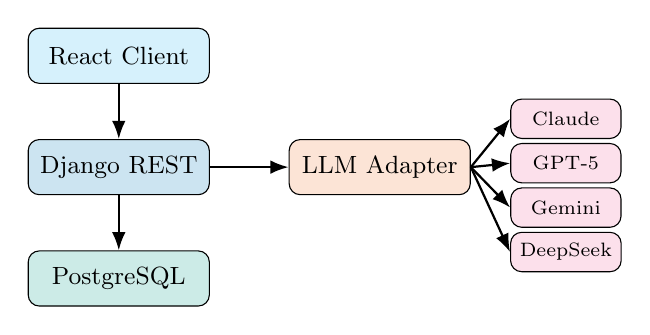
\begin{tikzpicture}[node distance=0.7cm,every node/.style={font=\small}]
    \node[draw,rounded corners,fill=vibrantcyan!20,minimum width=2.3cm,minimum height=0.7cm] (client) {React Client};
    \node[draw,rounded corners,fill=vibrantblue!20,minimum width=2.3cm,minimum height=0.7cm,below=of client] (api) {Django REST};
    \node[draw,rounded corners,fill=vibrantteal!20,minimum width=2.3cm,minimum height=0.7cm,below=of api] (db) {PostgreSQL};
    \node[draw,rounded corners,fill=vibrantorange!20,minimum width=2.3cm,minimum height=0.7cm,right=1.0cm of api] (adapter) {LLM Adapter};
    \node[draw,rounded corners,fill=vibrantmagenta!15,minimum width=1.4cm,minimum height=0.5cm,above right=0.0cm and 0.5cm of adapter] (claude) {\scriptsize Claude};
    \node[draw,rounded corners,fill=vibrantmagenta!15,minimum width=1.4cm,minimum height=0.5cm,below=0.05cm of claude] (gpt) {\scriptsize GPT-5};
    \node[draw,rounded corners,fill=vibrantmagenta!15,minimum width=1.4cm,minimum height=0.5cm,below=0.05cm of gpt] (gemini) {\scriptsize Gemini};
    \node[draw,rounded corners,fill=vibrantmagenta!15,minimum width=1.4cm,minimum height=0.5cm,below=0.05cm of gemini] (deepseek) {\scriptsize DeepSeek};
    \draw[-Latex,thick] (client) -- (api);
    \draw[-Latex,thick] (api) -- (db);
    \draw[-Latex,thick] (api) -- (adapter);
    \draw[-Latex,thick] (adapter.east) -- (claude.west);
    \draw[-Latex,thick] (adapter.east) -- (gpt.west);
    \draw[-Latex,thick] (adapter.east) -- (gemini.west);
    \draw[-Latex,thick] (adapter.east) -- (deepseek.west);
    \end{tikzpicture}
    \caption{SimilCode three-tier architecture with provider-agnostic LLM adapter.}
    \label{fig:architecture}
    \end{figure}
     
    \textbf{Development methodology.} Given the bounded scope and well-defined requirements, we adopted rapid prototyping \citep{tripp1990rapid,chang2025automatic}. Requirements were elicited through semi-structured interviews with five programming instructors (mean experience 8.4~years). The resulting specification follows ISO/IEC/IEEE~29148:2018 \citep{iso29148} and comprises 22 functional requirements grouped into five modules (individual comparison, group comparison, AI integration, language management, comparison administration), 9 non-functional requirements (performance, security, scalability), and 8 security/privacy requirements.
     
    \textbf{Modules.} The \emph{individual comparison} module accepts two code fragments, dispatches them to the selected LLM with the standardized prompt, parses the response, computes Big~O time and space complexity through static-flow inspection, and renders an integrated report. The \emph{group comparison} module generalizes to $n \geq 3$ fragments, computing the $\binom{n}{2}$ pairwise similarities and ranking efficiency. Big~O analysis is implemented as a hybrid: AST-derived loop-nesting depth and operation counting yield a candidate complexity, which the LLM validates and refines using its semantic understanding.
    \subsection{Expert Validation}
    After the comparative experiment and system implementation, five domain experts (instructors of programming courses, mean experience 6.8~years) participated in individual 45-minute sessions. Each session comprised a 10-minute system demonstration, 20 minutes of hands-on interaction with 10 representative code pairs, and a 15-minute structured questionnaire. The instrument comprised 18 Likert-scale items (1--5) across three sections --- practical usefulness (7 items), result accuracy (6 items), justification interpretability (5 items) --- plus two open-ended items. Sample size of five aligns with established usability-evaluation guidance \citep{kusmaryono2022number}, which finds that 3--5 evaluators suffice to surface most usability issues.
    \subsection{Ethical Considerations}
    The study followed standard research-ethics norms \citep{rodrigues2023ethical,resnik2024ethics}: informed consent was obtained from all participants, data were anonymized and reported in aggregate, LLM API usage complied with provider terms, and all evaluation code was either author-authored or in the public domain. Raw experimental data are archived for replicability.
    \section{Results}\label{sec:results}
    \subsection{Precision of Detection}
    Across the 480 trials, all four models classified 118 of 120 cases correctly, yielding identical mean precision of 98.3\%. Disaggregated by language: Claude Opus~4.1 and Gemini~2.5~Pro achieved 100\% in both C\# and Java; GPT-5 and DeepSeek-V3 reached 96.7\% in C\# (two structural-vs-functional confusions) and 100\% in Java. The one-way ANOVA returned $F(3,476) = 0.000$, $p = 1.000$, $\eta^2 < 0.001$, indicating no statistically detectable between-model variance. We therefore retain $H_{0,1}$: precision is equivalent across models. Figure~\ref{fig:precision} visualizes the result.
    \begin{figure}[!t]
    \centering
    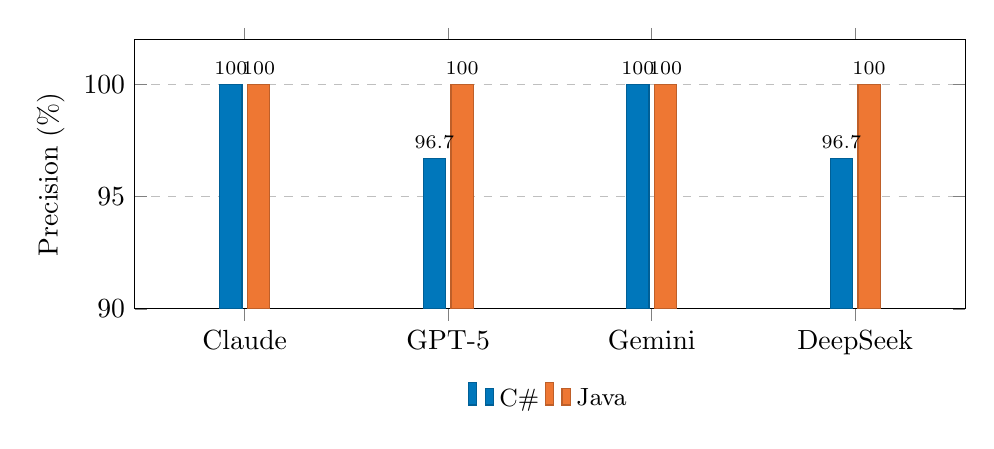
\begin{tikzpicture}
    \begin{axis}[width=\linewidth,height=5cm,ybar,bar width=8pt,enlarge x limits=0.18,ymin=90,ymax=102,
    ylabel={Precision (\%)},symbolic x coords={Claude,GPT-5,Gemini,DeepSeek},xtick=data,
    legend style={at={(0.5,-0.25)},anchor=north,legend columns=2,draw=none,font=\small},
    nodes near coords,nodes near coords align={vertical},nodes near coords style={font=\scriptsize},
    ymajorgrids=true,grid style=dashed]
    \addplot[fill=vibrantblue,draw=vibrantblue!80!black] coordinates {(Claude,100)(GPT-5,96.7)(Gemini,100)(DeepSeek,96.7)};
    \addplot[fill=vibrantorange,draw=vibrantorange!80!black] coordinates {(Claude,100)(GPT-5,100)(Gemini,100)(DeepSeek,100)};
    \legend{C\#,Java}
    \end{axis}
    \end{tikzpicture}
    \caption{Classification precision per model and language ($n=60$ per cell). All models exceed 96\% in both languages; ANOVA yields $p = 1.000$.}
    \label{fig:precision}
    \end{figure}
    \subsection{Response Time}
    Mean response times (s) and dispersion are reported in Table~\ref{tab:time}. Claude Opus~4.1 was fastest at 19.08~s overall, followed by DeepSeek-V3 (23.15~s), GPT-5 (24.72~s), and Gemini~2.5~Pro (25.73~s). The fastest-to-slowest gap of 6.65~s represents a 34.8\% relative latency increase. ANOVA returned $F(3,476) = 30.89$, $p < 0.001$, $\eta^2 = 0.163$ (large effect). Tukey HSD post-hoc indicated Claude Opus~4.1 differed significantly from each of the other three models ($p < 0.001$ in all three pairwise contrasts), while differences among GPT-5, Gemini, and DeepSeek were not all significant. We reject $H_{0,2}$ in favor of $H_{1,2}$.
    \begin{table}[!t]
    \caption{Response Time Statistics by Model (Seconds)}\label{tab:time}
    \centering\small
    \begin{tabular}{@{}lcccc@{}}\toprule
    Model & Mean & SD & CV (\%) & Range \\\midrule
    Claude Opus~4.1 & 19.08 & 2.41 & 12.6 & 14.2--26.1 \\
    DeepSeek-V3 & 23.15 & 3.88 & 16.8 & 16.7--32.9 \\
    GPT-5 & 24.72 & 3.62 & 14.6 & 17.4--34.0 \\
    Gemini~2.5~Pro & 25.73 & 4.11 & 16.0 & 18.0--35.6 \\\bottomrule
    \end{tabular}
    \end{table}
    \begin{figure}[!t]
    \centering
    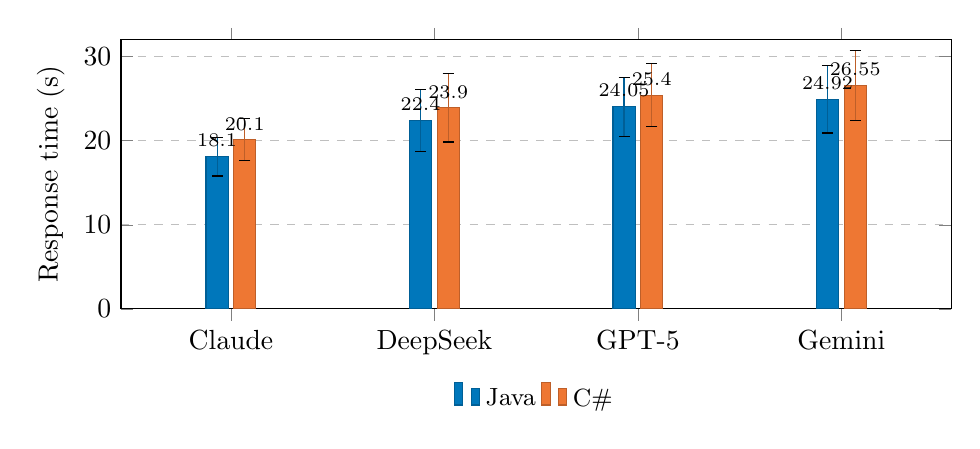
\begin{tikzpicture}
    \begin{axis}[width=\linewidth,height=5cm,ybar,bar width=8pt,enlarge x limits=0.18,ymin=0,ymax=32,
    ylabel={Response time (s)},symbolic x coords={Claude,DeepSeek,GPT-5,Gemini},xtick=data,
    legend style={at={(0.5,-0.25)},anchor=north,legend columns=2,draw=none,font=\small},
    nodes near coords,nodes near coords align={vertical},nodes near coords style={font=\scriptsize},
    ymajorgrids=true,grid style=dashed,
    error bars/y dir=both,error bars/y explicit]
    \addplot[fill=vibrantblue,draw=vibrantblue!80!black] plot[error bars/.cd,y dir=both,y explicit]
    coordinates {(Claude,18.10) +- (0,2.30) (DeepSeek,22.40) +- (0,3.70) (GPT-5,24.05) +- (0,3.50) (Gemini,24.92) +- (0,4.00)};
    \addplot[fill=vibrantorange,draw=vibrantorange!80!black] plot[error bars/.cd,y dir=both,y explicit]
    coordinates {(Claude,20.10) +- (0,2.50) (DeepSeek,23.90) +- (0,4.05) (GPT-5,25.40) +- (0,3.75) (Gemini,26.55) +- (0,4.20)};
    \legend{Java,C\#}
    \end{axis}
    \end{tikzpicture}
    \caption{Mean response time per model and language with $\pm 1$~SD error bars. Claude Opus~4.1 is significantly faster than all alternatives (Tukey HSD $p < 0.001$).}
    \label{fig:time}
    \end{figure}
    \subsection{Justification Quality}
    Composite quality scores (range 0--5) are summarized in Table~\ref{tab:quality}. Claude Opus~4.1 obtained the highest mean (4.96), followed by Gemini~2.5~Pro (4.92), GPT-5 (4.85), and DeepSeek-V3 (4.83). Kruskal--Wallis returned $H = 11.50$, $p = 0.009$, $\epsilon^2 = 0.024$. Dunn's post-hoc with Bonferroni correction indicated Claude differed significantly from DeepSeek-V3 ($p = 0.012$) and from GPT-5 ($p = 0.041$); other contrasts were non-significant. We reject $H_{0,3}$ in favor of $H_{1,3}$.
    \begin{table}[!t]
    \caption{Justification Quality by Dimension and Model (Mean, 1--5 Scale)}\label{tab:quality}
    \centering\small
    \begin{tabular}{@{}lcccc@{}}\toprule
    Dimension & Claude & GPT-5 & Gemini & DeepSeek \\\midrule
    Clarity & 4.97 & 4.86 & 4.93 & 4.81 \\
    Completeness & 4.95 & 4.84 & 4.90 & 4.82 \\
    Coherence & 4.96 & 4.85 & 4.93 & 4.86 \\\midrule
    Composite & \textbf{4.96} & 4.85 & 4.92 & 4.83 \\\bottomrule
    \end{tabular}
    \end{table}
    \begin{figure}[!t]
    \centering
    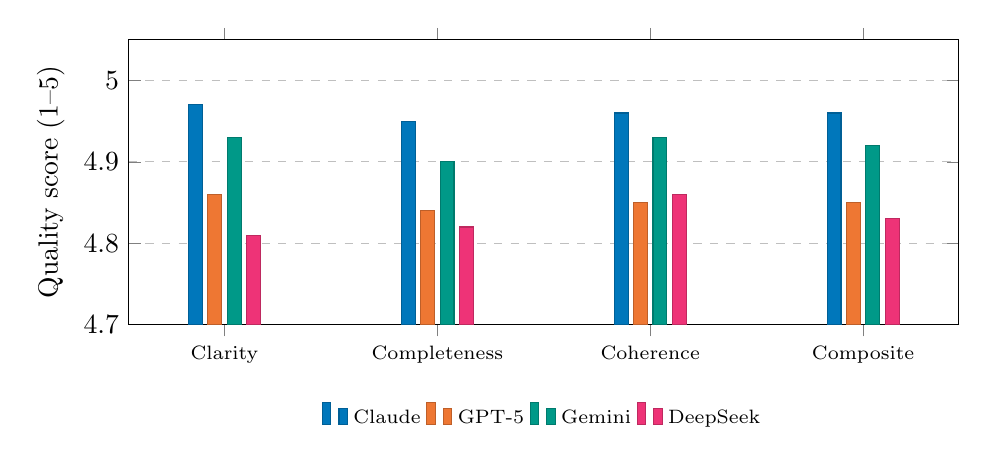
\begin{tikzpicture}
    \begin{axis}[width=\linewidth,height=5.2cm,ybar=2pt,bar width=5pt,enlarge x limits=0.15,
    ymin=4.7,ymax=5.05,ylabel={Quality score (1--5)},
    symbolic x coords={Clarity,Completeness,Coherence,Composite},xtick=data,
    xticklabel style={font=\scriptsize},
    legend style={at={(0.5,-0.25)},anchor=north,legend columns=4,draw=none,font=\scriptsize},
    ymajorgrids=true,grid style=dashed]
    \addplot[fill=vibrantblue,draw=vibrantblue!80!black] coordinates {(Clarity,4.97)(Completeness,4.95)(Coherence,4.96)(Composite,4.96)};
    \addplot[fill=vibrantorange,draw=vibrantorange!80!black] coordinates {(Clarity,4.86)(Completeness,4.84)(Coherence,4.85)(Composite,4.85)};
    \addplot[fill=vibrantteal,draw=vibrantteal!80!black] coordinates {(Clarity,4.93)(Completeness,4.90)(Coherence,4.93)(Composite,4.92)};
    \addplot[fill=vibrantmagenta,draw=vibrantmagenta!80!black] coordinates {(Clarity,4.81)(Completeness,4.82)(Coherence,4.86)(Composite,4.83)};
    \legend{Claude,GPT-5,Gemini,DeepSeek}
    \end{axis}
    \end{tikzpicture}
    \caption{Justification quality across rubric dimensions. Claude Opus~4.1 leads in all dimensions; differences are significant against DeepSeek and GPT-5.}
    \label{fig:quality}
    \end{figure}
    \subsection{Consolidated Hypothesis Tests}
    Table~\ref{tab:hypotheses} summarizes the inferential results. Two of three specific hypotheses are rejected, supporting the general conclusion that performance differences between LLMs are detectable, with Claude Opus~4.1 dominating on operational dimensions despite precision parity.
    \begin{table*}[!t]
    \caption{Summary of Hypothesis Tests}\label{tab:hypotheses}
    \centering\small
    \begin{tabular}{@{}llccc@{}}\toprule
    Hypothesis & Test & Statistic & $p$ & Decision \\\midrule
    $H_{0,1}$ Precision & ANOVA & $F = 0.00$ & 1.000 & Retain \\
    $H_{0,2}$ Time & ANOVA & $F = 30.89$ & $<.001$ & Reject \\
    $H_{0,3}$ Quality & Kruskal--Wallis & $H = 11.50$ & 0.009 & Reject \\\bottomrule
    \end{tabular}
    \end{table*}
    \subsection{System Functional Output}
    Figure~\ref{fig:simoutput} schematically illustrates the integrated output of the individual-comparison module: a five-dimensional similarity profile plus per-fragment Big~O classification. For an illustrative pair of bubble-sort variants, the system reported lexical~76, structural~88, stylistic~64, functional~95, syntactic~82, global~83 --- and identified both fragments as $\mathcal{O}(n^2)$ time / $\mathcal{O}(1)$ space, with fragment~B marginally more efficient due to the absence of a redundant inner condition.
    \begin{figure}[!t]
    \centering
    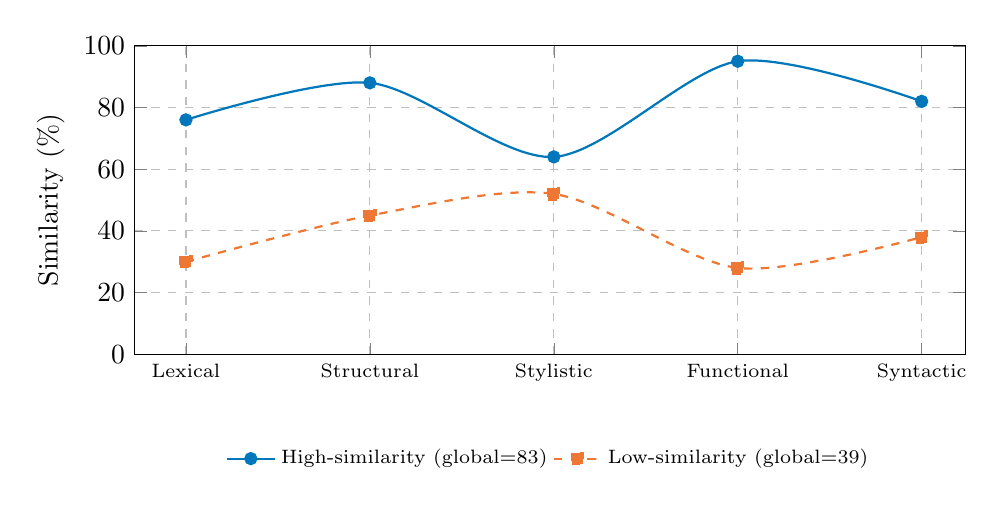
\begin{tikzpicture}
    \begin{axis}[width=\linewidth,height=5.5cm,
    xtick={0,72,144,216,288},xticklabels={Lexical,Structural,Stylistic,Functional,Syntactic},
    ymin=0,ymax=100,ylabel={Similarity (\%)},xmin=-20,xmax=305,
    ymajorgrids=true,xmajorgrids=true,grid style=dashed,
    legend style={at={(0.5,-0.27)},anchor=north,legend columns=2,draw=none,font=\scriptsize},
    xticklabel style={font=\scriptsize}]
    \addplot[smooth,thick,vibrantblue,mark=*,mark options={fill=vibrantblue}] coordinates {(0,76)(72,88)(144,64)(216,95)(288,82)};
    \addplot[smooth,thick,vibrantorange,dashed,mark=square*,mark options={fill=vibrantorange}] coordinates {(0,30)(72,45)(144,52)(216,28)(288,38)};
    \legend{High-similarity (global=83),Low-similarity (global=39)}
    \end{axis}
    \end{tikzpicture}
    \caption{Five-dimensional similarity profile output by the SimilCode individual-comparison module for two illustrative pairs.}
    \label{fig:simoutput}
    \end{figure}
    \begin{figure}[!t]
    \centering
    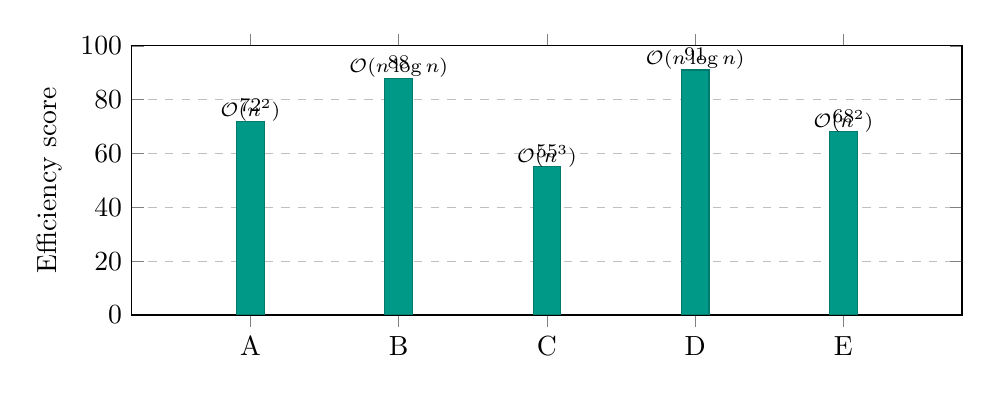
\begin{tikzpicture}
    \begin{axis}[width=\linewidth,height=5cm,
    ybar,bar width=10pt,enlarge x limits=0.2,ymin=0,ymax=100,
    ylabel={Efficiency score},symbolic x coords={A,B,C,D,E},xtick=data,
    nodes near coords,nodes near coords align={vertical},nodes near coords style={font=\scriptsize},
    ymajorgrids=true,grid style=dashed]
    \addplot[fill=vibrantteal,draw=vibrantteal!80!black] coordinates {(A,72)(B,88)(C,55)(D,91)(E,68)};
    \node[font=\scriptsize] at (axis cs:A,76){$\mathcal{O}(n^2)$};
    \node[font=\scriptsize] at (axis cs:B,92){$\mathcal{O}(n\log n)$};
    \node[font=\scriptsize] at (axis cs:C,59){$\mathcal{O}(n^3)$};
    \node[font=\scriptsize] at (axis cs:D,95){$\mathcal{O}(n\log n)$};
    \node[font=\scriptsize] at (axis cs:E,72){$\mathcal{O}(n^2)$};
    \end{axis}
    \end{tikzpicture}
    \caption{Group-comparison module: efficiency ranking for a 5-fragment cohort with annotated Big~O complexities. Fragment~D leads.}
    \label{fig:groupout}
    \end{figure}
    \subsection{Expert Validation}
    The five experts produced a global mean of 4.60/5.00 (Table~\ref{tab:experts}). Practical-usefulness items obtained the highest section mean (4.80), driven by perfect or near-perfect scores on similarity detection, Big~O usefulness, and intent-to-adopt. Result-accuracy averaged 4.60, with the identical-pair detection item reaching 5.00 across all experts. Justification-interpretability averaged 4.60, with the score-explanation item also at 5.00. Open-ended feedback emphasized the value of integrating efficiency and similarity in a single screen and requested support for additional languages.
    \begin{table}[!t]
    \caption{Expert Validation Results (1--5 Likert)}\label{tab:experts}
    \centering\small
    \begin{tabular}{@{}lcccc@{}}\toprule
    Expert & Usefulness & Accuracy & Interpret. & Mean \\\midrule
    E1 & 5 & 5 & 4 & 4.75 \\
    E2 & 5 & 4 & 5 & 4.50 \\
    E3 & 4 & 5 & 5 & 4.75 \\
    E4 & 5 & 4 & 4 & 4.25 \\
    E5 & 5 & 5 & 5 & 4.75 \\\midrule
    Mean & 4.80 & 4.60 & 4.60 & \textbf{4.60} \\\bottomrule
    \end{tabular}
    \end{table}
    \section{Discussion}\label{sec:discussion}
    The findings refine and extend the literature in three directions. The first direction concerns precision parity. The equivalent precision observed across four leading commercial LLMs aligns with the maturation trend documented by \citet{zhang2025machine} for ML-based similarity detection, and extends it to general-purpose foundation models that lack code-specific training. Practically, this implies that institutions should not select among modern LLMs on precision grounds alone --- a result that simplifies procurement but reframes selection toward operational metrics.
     
    The 6.65~s latency gap between Claude Opus~4.1 and Gemini~2.5~Pro becomes economically meaningful at institutional scale. In a course of 200 students with 10 weekly submissions, the cumulative delta exceeds 3.7~hours per week, validating \citet{franclinton2020scalable}'s emphasis on temporal scalability. This finding suggests that response time, often treated as a secondary concern in educational AI research, should be elevated to a primary selection criterion when LLMs are deployed at scale.
     
    The second direction concerns the quality of LLM-generated explanations. The differential observed in our experiments aligns with \citet{keuning2018systematic}'s finding that automated-feedback usefulness depends critically on clarity. Our composite quality differences are numerically small but statistically significant. Qualitative inspection of justifications further indicates that the differences manifest in technical specificity: Claude tends to cite concrete control-flow constructs, while DeepSeek occasionally produces generic phrasings. For educational deployment --- where justifications are directly read by students --- this margin is non-trivial.
     
    The CoT/CoVe-engineered prompt likely contributes to the high absolute scores observed for all models, consistent with \citet{wei2022chain} and \citet{dhuliawala2024chain}. This suggests that prompt engineering may compress the quality gap between LLMs even when the models differ substantially in underlying capabilities, although the residual gap remains statistically detectable.
     
    The third direction concerns the integration of similarity and efficiency analysis. The unified workflow proposed in this study addresses a gap identified across multiple reviews \citep{lee2023review,zakeri2023systematic,zviel2024good}. Existing tools either detect plagiarism (MOSS, JPlag) or analyze quality (PMD, SonarQube), but not both. The expert-validation result (4.80/5 on usefulness, with 5/5 on Big~O usefulness) provides empirical support for this design decision, complementing \citet{manorat2025artificial}'s observation that AI-in-education research over-emphasizes assistance over assessment.
     
    \textbf{Limitations.} Three limitations bound the generalizability of these findings. The first is dataset coverage: the experimental corpus is restricted to C\# and Java, and results may differ for languages with distinct paradigms (Python's dynamic typing, C++'s template metaprogramming). The second is model evolution: LLMs evolve rapidly, and the specific model versions tested in 2025 may be superseded; we mitigate this via the provider-agnostic adapter, which permits straightforward re-benchmarking. The third is sample size in expert validation: $n=5$ aligns with usability heuristics \citep{kusmaryono2022number} but does not capture institutional-scale adoption dynamics, and future work should include longitudinal studies in real classrooms.
     
    \textbf{Implications.} The system architecture and evaluation protocol are reusable beyond the immediate study. The standardized prompt and rubric can serve as benchmarks for future LLMs, and the adapter pattern permits incremental integration of new providers. For research on AI-augmented programming education, the results motivate a shift from reporting precision in isolation to multidimensional evaluation that prioritizes latency and explanation quality.
    \section{Conclusions}\label{sec:conclusion}
    This work contributes empirical, methodological, and engineering advances to the intersection of LLMs and software-engineering education. Empirically, four state-of-the-art commercial LLMs achieve equivalent precision (98.3\%) on multidimensional code-similarity detection. They differ significantly in latency (Claude Opus~4.1 fastest at 19.08~s) and in justification quality (Claude Opus~4.1 highest at 4.96/5). Methodologically, the CoT/CoVe-engineered prompt and three-axis rubric provide a reproducible benchmark for future LLM evaluations on code-comparison tasks.
     
    As an engineering artifact, SimilCode integrates five-dimensional semantic similarity with automated Big~O efficiency analysis in a single deployable web application. It addresses a documented gap in academic code-evaluation tooling and was validated by expert instructors at 4.60/5.00.
     
    Future work will pursue four directions. First, evaluation will be extended to Python, JavaScript, and C++ to assess language-paradigm effects on LLM performance. Second, a public benchmark with verified-complexity reference algorithms will be established for systematic Big~O validation. Third, longitudinal classroom studies will measure learning outcomes attributable to the system. Fourth, a continuous-evaluation protocol will be implemented to update LLM rankings as new model versions are released.
    \section*{Acknowledgments}
    The authors thank the five expert instructors who contributed to system validation, and the Faculty of Computer Sciences of Universidad T\'ecnica Estatal de Quevedo for institutional support.
    \section*{Conflict of Interest}
    The authors declare no conflict of interest.
    \bibliographystyle{unsrtnat}
    \bibliography{references}
\end{document}